\paragraph{Bagging}
\subparagraph{Bootstrap aggregation (bagging) definition}
It is a \tB{general-purpose procedure for reducing the variance of a
statistical learning method}; we introduce it here because it is
particularly useful and frequently used in the context of decision
trees.\\
In other words for estimating $\hat{f}(x)$, the prediction at input x, we could calculate $\left(f^{i
}(x)\right)_{1\leq i\leq B}$ using $B$ separate training sets, and average them in order to
obtain a single low-variance statistical learning model.\\
We then \sB{train our method on the $b^{th}$ bootstrapped training set in
order to get $\hat{f}^{*b}(x)$}, and finally average all the predictions
to obtain:
\begin{center}
	\encB{$\hat{f}_{bag}(x)=\dfrac{1}{B}\su{{b=1}}{B}\hat{f}^{*b}(x)$}
\end{center}
This is called bagging.

\emph{Python Code}
\begin{python}
import pandas as pd
import sklearn
from sklearn import tree
from sklearn.ensemble import BaggingClassifier,
    BaggingRegressor

y, X = df.iloc[:, 0], df.iloc[:, 1:]
bagging = BaggingClassifier(tree.DecisionTreeClassifier(),
    max_samples=0.5, max_features=0.5)
\end{python}

\subparagraph{Out-of-Bag Error Estimation}
The key to bagging is that trees are repeatedly fit to bootstrapped subsets of the observations.

\paragraph{Random Forest}
When building these decision trees, \sR{each time a split in a tree is 
considered, a random sample of $m$ predictors is chosen as split 
candidates from the full set of $p$ predictors}.\\
In building a random forest, at each split in the tree the algorithm
is \emph{not even allowed to consider} a majority of the available
predictors.

\subparagraph{Random Forest for Regression or Classification}
\begin{enumerate}
	\item For $b\in\inter{1}{B}$
		\begin{enumerate}[label=(\alph*)]
			\item \sB{Draw a bootstrap sample $\bm{Z}^{*}$ of size $N$} from the training
				data
			\item \sB{Grow a random-forest tree $T_{b}$ to the bootstrapped data}, by
				recursively repeating the following steps for each terminal mode
				of the tree, until the minimum node size $n_{min}$ is reached.
				\begin{enumerate}[label=\alph*]
					\item[i.] Select $m$ variables at random from the $p$ 
						variables
					\item[ii.] Pick the best variable/split-point among the $m$
					\item[iii.] Split the node into 2 daughter nodes.
				\end{enumerate}
		\end{enumerate}
	\item Output the ensemble of trees $\left\{T_{b}\right\}_{1}^{B}$
\end{enumerate}
\textit{Regression}: \enc{$\hat{f}_{rf}^{B}(x) = \dfrac{1}{B}\su{{b=1}}{B}T_{b}(x)$}\\
\textit{Classification}: Let $\hat{C}_{b}(x)$ be the class prediction of the $b^{th}$ 
random-forest tree, then $\hat{C}_{rf}^{B}(x)=majority\_vote\left\{\hat{C}_{b}(x)\right\}_{1}^{B}$

\subparagraph{Python Code}
\begin{python}
import pandas as pd
import sklearn
from sklearn.ensemble import RandomForestClassifier,
    RandomForestRegressor

y, X = df.iloc[:, 0], df.iloc[:, 1:]
clf = RandomForestClassifier(n_estimator=10)
\end{python}

\paragraph{Boosting}
\subparagraph{Boosting for Regression Trees}
The motivation for boosting was a procedure that combines the outputs of many ``weak'' classifiers
to produce a powerful ``committee'''. A \sB{weak classifier is one whose error rate is only slightly
better than random guessing}.
\begin{enumerate}
	\item Set $\hat{f}(x)=0$ and $r_{i}=y_{i}$ for all $i$ in the
		training set.
	\item For $b\in\inter{1}{B}$ repeat:
		\begin{enumerate}[label=\alph*]
			\item Fit a tree $\hat{f}^{b}$ with $d$ splits
				($d+1$ terminal nodes) to the training
				data (X,r)
			\item Update $\hat{f}$ by adding in a shrunken
				version of the new tree:
				$$
				\hat{f}(x)\leftarrow \hat{f}(x)+\lambda
				\hat{f}^{b}(x)
				$$
			\item Update the residuals,
				$r_{i}\leftarrow r_{i}-\lambda \hat{f}^{b}(x_{i})$
			\end{enumerate}
	\item Output the boosted model, $\hat{f}(x)=\su{{b=1}}{B}\lambda\hat{f}^{b}(x)$
\end{enumerate}

\subparagraph{Boosting methods}
Consider a two-class problem, with the output variable coded as $Y\in\left\{-1,1\right\}$. Given a
vector of predictor variables $X$, a classifier $G(X)$ produces a prediction taking one of the 
2 values $\{-1,1\}$
\begin{figure}[H]
	\begin{center}
		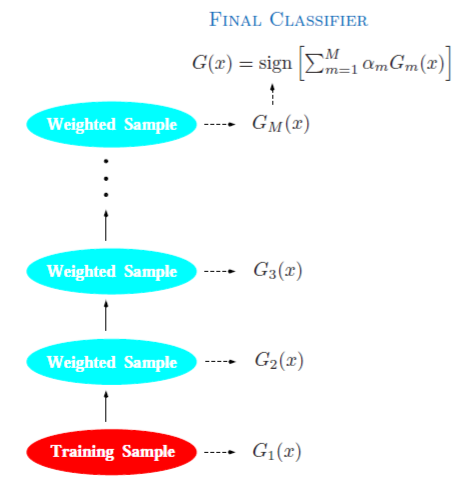
\includegraphics[width=.5\textwidth]{./chap/1chap/7sec/images/1_adaboost.PNG}
	\end{center}
	\caption{Schematic of AdaBoost. Classifiers are trained on weighted versions of the 
	dataset, and then combined to produce a final prediction.}
	\label{fig:1_adaboost}
\end{figure}
\begin{center}
	\encB{$ G(x) = sign\left( \su{{m=1}}{M}\alpha_{m}G_{m}(x) \right)$}
\end{center}
Here \sB{$\alpha_{m}$'s are computed by the boosting algorithm and weight the contribution of each 
respective $G_{m}(x)$}. Their effect is to give higher influence to the more accurate classifiers in
the sequence.

\subparagraph{AdaBoost.M1}
\begin{enumerate}
	\item Initialize the observation weights $w_{i}=\frac{1}{N}, i\in\inter{1}{N}$
	\item For $m\in\inter{1}{M}$:
		\begin{enumerate}[label=\alph*]
			\item Fit a classifier $G_{m}(x)$ to the training data using weights $w_{i}$
			\item Compute:
				$$ err_{m} = \dfrac{\su{{i=1}}{N}\omega_{i}I\left(y_{i}\neq G_{m}(x_{i})\right)}{\su{{i=1}}{N}\omega_{i}}$$
			\item Compute \tV{$\alpha_{m}=\log\left(\dfrac{1-err_{m}}{err_{m}}\right)$}
			\item Set \tV{$\omega_{i} \leftarrow \omega_{i}e^{\alpha_{m}I(y_{i}\neq G_{m}(x_{i}))}$ for $i\in\inter{1}{N}$}
		\end{enumerate}
	\item Output $G(x)=sign\left[\su{{m=1}}{M}\alpha_{m}G_{m}(x)\right]$
\end{enumerate}
\subparagraph{Python Code}
\begin{python}
import pandas as pd
import sklearn
from sklearn.ensemble import AdaBoostClassifier,
    AdaboostRegressor
from sklearn.model_selection import corss_val_score

y, X = df.iloc[:, 0], df.iloc[:, 1:]
clf = AdaBoostClassifier(n_estimator=100)
scores = corss_val_score(clf, X, y, cv=5)
\end{python}

\paragraph{Boosting Fits an Additive Model}
\begin{center}
\encB{$ f(x)=\su{{m=1}}{M}\beta_{m}b(x;\gamma_{m})$}
\end{center}
where $\beta_{m}$'s are the expansion coefficients and $b(x;\gamma)\in\mathbb{R}$ are usually
simple functions of the multivariate argument $x$, characterized by a set of parameters $\gamma$
\subparagraph{Forward Stagewise Additive Modeling}
\begin{enumerate}
	\item Initialize $f_{0}(x)=0$
	\item For $m\in\inter{1}{M}$
		\begin{enumerate}[label=\alph*]
			\item Compute \tV{$(\beta_{m},\gamma_{m}) = \min\limits_{\beta,\gamma}\su{{i=1}}{N}L(y_{i},f_{m-1}(x_{i})+\beta b(x_{i};\gamma))$}
			\item Set $f_{m}(x)=f_{m-1}(x)+\beta_{m}b(x;\gamma_{m})$
		\end{enumerate}
\end{enumerate}

\paragraph{Forward Stagewise Additive Modeling}
\sB{At each iteration $m$, one solves the optimal basis function $b(x;\gamma_{m})$ and corresponding
coefficient $\beta_{m}$ to add the current expansion $f_{m-1}(x)$.} This procedure $f_{m}(x)$,
and the process is repeated.
For the squared-error loss: $L(y,f(x))=\left(y-f(x)\right)^{2}$ one has 
\begin{align*}
L(y_{i},f_{m-1}(x_{i})+\beta b(x_{i};\gamma)) =& \left(y_{i}-f_{m-1}(x)-\beta 
b(x_{i};\gamma)\right)\\
=& \left(r_{im}-\beta b(x_{i},\gamma)\right)^{2}
\end{align*}
where $r_{im}=y_{i}-f_{m-1}(x_{i})$ is simply the residual of the current model on the $i^{th}$
observation.

\paragraph{Loss Functions and Robustness}
\subparagraph{Robust Loss Functions for Classification}
The minimizer of the corresponding risk on the population is :
$$ f^{*}(x)=\min\limits_{f(x)}\mathbb{E}_{Y|x}\left(Y-f(x)\right)^{2} = \E{Y|X}=2\ProbC{x}{Y=1}
-1$$
\begin{figure}[H]
	\begin{center}
		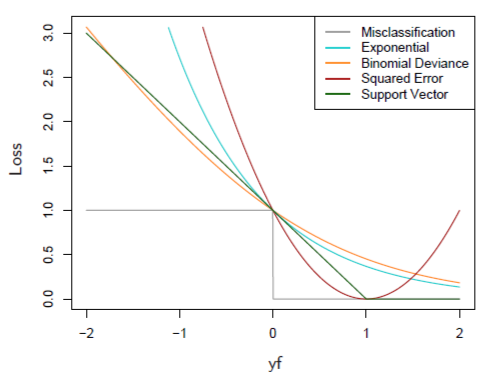
\includegraphics[width=.6\textwidth]{./chap/1chap/7sec/images/2_LossFunction.PNG}
	\end{center}
	\caption{The response is $y=\pm 1$ the prediction is $f$, with class prediction $sign(f)$.
	The losses are misclassification: $I(sign(f)\neq y)$; exponential: $exp(-yf)$; binomial
	deviance $\log(1+e^{-2yf})$; squared error $(y-f)^{2}$; and support vector: $(1-yf)_{+}$}
	\label{fig:2_LossFunction}
\end{figure}
\subparagraph{Python Code}
\begin{python}
import pandas as pd
import sklearn
from sklearn.ensemble import GradientBoostingClassifier
from sklearn.model_selection import train_test_split

y, X = df.iloc[:, 0], df.iloc[:, 1:]
X_train, X_test, y_train, y_test = train_test_split(
    X, y, random_state=0)
clf = GradientBoostingClassifier(
   loss = 'deviance', # {'deviance', 'exponential'}
   random_state = 0
)
print(clf.score(X_test, y_test))
\end{python}
\subparagraph{Robust Loss Functions for Regression}
One such criterion is the Huber loss criterion used for M-regression
$$ L(y,f(x))=
\begin{cases}
	\left(y-f(x)\right)^{2} \Leftarrow |y-f(x)|\leq \delta \\
	2\delta|y-f(x)|-\delta^{2} \Leftarrow |y-f(x)|> \delta
\end{cases}
$$
\begin{figure}[H]
	\begin{center}
		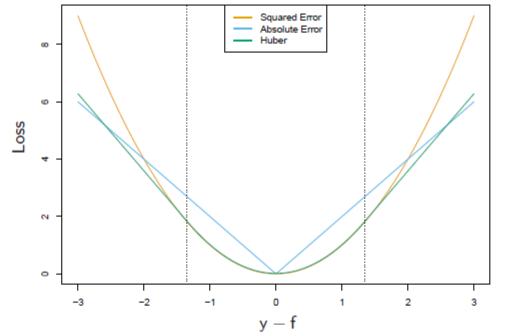
\includegraphics[width=.7\textwidth]{./chap/1chap/7sec/images/3_LossFunction_reg.PNG}
	\end{center}
	\caption{The Huber loss function combines the good properties of squared-error loss near
	zero and absolute error loss when $|y-f|$ is large}
	\label{fig:3_LossFunction_reg}
\end{figure}

\subparagraph{Python Code}
\begin{python}
import pandas as pd
import sklearn
from sklearn.ensemble import GradientBoostingRegressor
from sklearn.model_selection import train_test_split

y, X = df.iloc[:, 0], df.iloc[:, 1:]
X_train, X_test, y_train, y_test = train_test_split(
    X, y, random_state=0)
reg = GradientBoostingRegressor(
   loss = 'huber', # {'ls', 'lad', 'huber'}
   random_state = 0
)
print(reg.score(X_test, y_test))
\end{python}



\paragraph{Procedures for Data Mining}
\begin{figure}[H]
	\begin{center}
		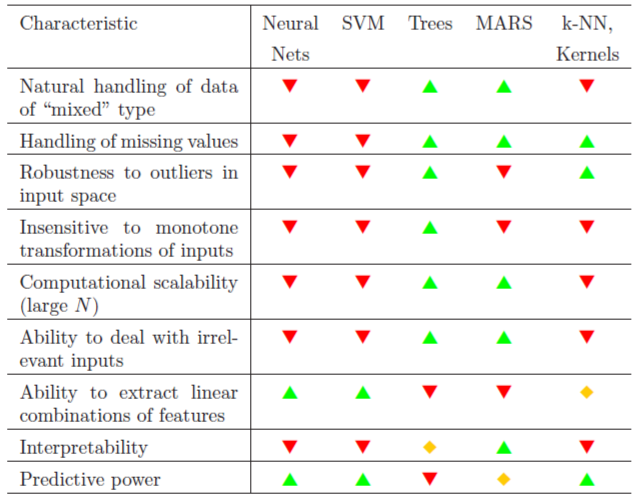
\includegraphics[width=\textwidth]{./chap/1chap/7sec/images/4_compMeth.PNG}
	\end{center}
	\caption{Some characteristics of different learning methods.Green=good, Yellow=fair, 
	Red=poor}
	\label{fig:4_compMeth}
\end{figure}

\paragraph{Boosting Trees}
Regression and classification trees partition the space of all joint predictor variable values
into disjoint regions $R_{j},j\in\inter{1}{J}$ as represented by the terminal nodes of the tree.\\
A constant $\gamma_{j}$ is assigned to each such region and the predictive rule is :
$x\in R_{j} \Rightarrow f(x)=\gamma_{j}$. Thus a tree can be formally expressed as:
$$ T(x;\Theta)=\su{{j=1}}{J}\gamma_{j}I(x\in R_{J})$$
with parameters $\Theta=\left\{R_{j},\gamma_{j}\right\}_{1}^{J}$
The parameters are found by minimizing the empirical risk: 
$\Theta = \min\limits_{\Theta}\su{{j=1}}{J}\su{{x_{i}\in R_{j}}}{}L(y_{i},\gamma_{j})$

\paragraph{Numerical Optimization via Gradient Boosting}
The goal is to minimize $L(f)=\su{{i=1}}{N}L(y_{i},f(x_{i}))$ with respect to $f$, where here
$f(x)$ is constrained to be a sum of trees. Ignoring this constraint, minimizing $L(f)$ can be
viewed as a numerical optimization:
$$ \hat{\bm{f}} = \min\limits_{f}L(\bm{f})$$ where the parameters $\bm{f}\in\mathbb{R}^{N}$ are
the values of the approximating function $f(x_{i})$ such as $\bm{f} = \left(f(x_{i})
\right)_{1\leq i\leq N}^{T}$
Numerical optimization procedures solves the previous equation as a sum of component vectors:
$$ \bm{f}_{M} = \su{{m=0}}{M}\bm{h}_{m}, \bm{h}_{m}\in\mathbb{R}^{N}$$

\subparagraph{Steepest Descent}
Steepest descent chooses \tB{$\bm{h}_{m} = -\rho_{m}\bm{g}_{m}, (\rho_{m}, \bm{g}_{m})\in\mathbb{R}
\times\mathbb{R}^{N}$, $\bm{g}_{m}$ is the gradient of $L(\bm{f})$ evaluated at $\bm{f}=\bm{f}_{
m-1}$}. The components of the gradient $\bm{g}_{m}$ are: 
\begin{center}
\encB{$ g_{im} = \left[\dfrac{\partial L(y_{i},f(x_{i}))}{\partial f(x_{i})}\right]_{f(x_{i}=f_{m-1}(
x_{1}))}$} 
\end{center}
The step length $\rho_{m}$ is the solution to 
$ \rho_{m}=\min\limits_{\rho}L\left(\bm{f}_{m-1}-\rho\bm{g}_{m}\right)$, the current solution
is then updated 
\begin{center}
	\enc{$ \bm{f}_{m} = \bm{f}_{m-1} -\rho_{m}\bm{g}_{m}$}
\end{center}

\begin{figure}[H]
	\begin{center}
		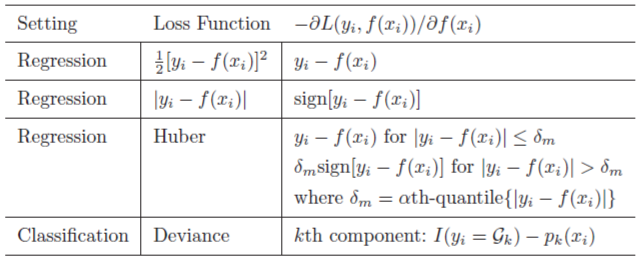
\includegraphics[width=\textwidth]{./chap/1chap/7sec/images/5_common_gradients.PNG}
	\end{center}
	\caption{Gradients for commonly used loss functions}
	\label{fig:5_common_gradients}
\end{figure}

Gradient Tree Boosting Algorithm
\begin{enumerate}
	\item Initialize $f_{0}(x)=\min\limits_{\gamma}\su{{i=1}}{N}L(y_{i},\gamma)$
	\item For $m\in\inter{1}{M}$:
		\begin{enumerate}[label=(\alph*)]
			\item For $i\in\inter{1}{N}$ compute: $r_{im}=-\left[\dfrac{\partial L(y_{i},f(x_{i}))}{\partial f(x_{i})}\right]_{f=f_{m-1}}$
			\item  Fit a regression tree to the targets $r_{im}$ giving terminal 
				regions $R_{jm},j\in\inter{1}{J_{m}}$
			\item For $j\in\inter{1}{J_{m}}$ compute: $\gamma_{jm}=\min\limits_{
				\gamma}\su{{x_{i}}\in R_{jm}}{}L(y_{i},f_{m-1}(x_{i}) + \gamma)$
			\item Update $f_{m}(x)=f_{m-1}(x)+\su{{j=1}}{J_{m}}\gamma_{jm}I(x\in\mathbb{R}_{jm})$
		\end{enumerate}
	\item Output $\hat{f}(x)=f_{M}(x)$
\end{enumerate}

